\chapter{Automatic Metadata Extraction and Update}
\graphicspath{{figs/04-extraction-update/}}

As we have an application ready to receive and display metadata, it is now crucial to turn the attention to extracting metadata from \gls{cdm} databases, which contain the actual data, allowing, then, to update the data stored on applications such as the MONTRA framework.

Figure \ref{fig:overall-arch-v1} presents a high-level architecture of the desired system that extracts data from databases and sends it to the applications that need their local data updated.
Agents are software that runs on the data owner's deployment, in charge of extracting metadata from the database and sending this metadata to the applications.

\begin{figure}[h]
    \center
    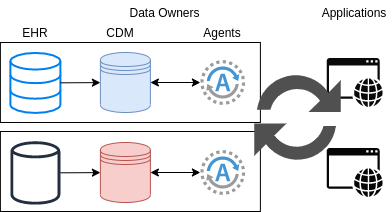
\includegraphics[width=.6\textwidth]{overall-arch-v1}
    \caption{High-level architecture of the extraction and update process.}
    \label{fig:overall-arch-v1}
\end{figure}

\section{Requirement Analysis}

When we enter the realm of accessing an institution's sensitive data, some problems start to arise.
Not all data owners are willing to, or legally can't, provide direct access to their data.
When building this part of the system, we have to consider this and have several options available that use different levels of access and according to the demands of each specific data owner, use the most appropriate one.
In one end, a single solution could have full access to the data, extracting the metadata directly from the original data.
At the other end of the scale, the burden of extracting data is removed from us and the system is dependent on the data owner providing the metadata and only then the system processes the metadata.
Having several options for different access levels is more flexible, however, it requires maintaining several tools which are not reliable.
A more appropriate alternative is to have a single option, that is designed considering the most strict access to the data, however, we still need to provide a tool to extract the metadata.
The only difference is that we are not the ones executing it.

As the extracting tool has direct access to the data, using an existing and widely known tool is a must, so data owners are inclined to use it.
Additionally, making fewer to no changes is preferable to ensure that data owners don't discard the tool because they don't trust the changes.

\begin{figure}[h]
    \center
    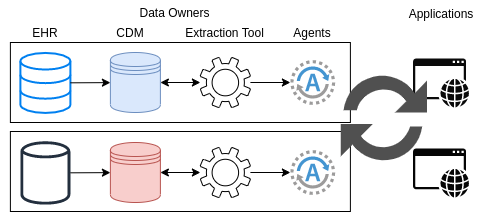
\includegraphics[width=.6\textwidth]{overall-arch-v2}
    \caption{High-level architecture of the extraction and update process}
    \label{fig:overall-arch-v2}
\end{figure}

In figure \ref{fig:overall-arch-v2} is presented the overall architecture of the system, where the agent is the tool in charge of parsing the metadata provided by the data owner, which is then sent to the applications.
Regarding this last point, there needs to be a way for the data to go from the agents to the applications.
One ambitious solution is to create a decentralized peer-to-peer network of agents, avoiding developing a central component.
In such solution, the agents are in charge of managing and sending the data to the applications.
However, data owners might not want to spend their hardware resources to maintain a network.
Since the agents are executed on the data owner's system, they should do only the required and minimal functionality, spending the few resources as possible.

A more executable solution is to have an intermediate component that receives the metadata from the agents and then distributes that data across the applications, following a centralized network architecture as it is presented in figure \ref{fig:overall-arch-v2}.

\begin{figure}[h]
    \center
    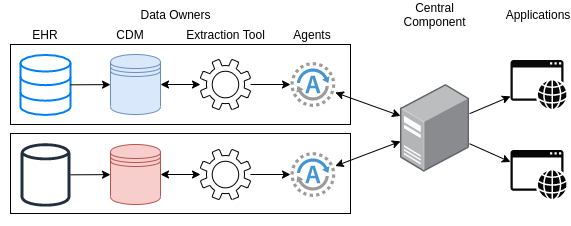
\includegraphics[width=.6\textwidth]{overall-arch-v3}
    \caption{High-level architecture of the extraction and update process, with a centralized network approach.}
    \label{fig:overall-arch-v3}
\end{figure}

This central component will be used to manage the data and the applications to where such has to be sent.
However, it is also crucial that feedback is provided on the system's state, such as how the data is flowing, which applications received which data, and which databases sent data into the system.

% aqui digo que percisamos de um componente intermedio. mais á frente vou dizer que percisamos um componente intermedio entre o kafka e as aplicações. coisas diferentes

On the applications side, there are other important factors to consider before going forward on implementing the intermediary component mentioned before.
First, the \gls{api}s of different applications expect the metadata in distinct arrangements.
A way out of this would be to specify a set of endpoints that each application had to implement, yet that would lead the applications to have two sets of endpoints that do the same thing.
On the other side, making a flexible option, where the requests where the data is sent are customizable, would be more appealing for the target applications, which would not have to make any changes.
Second, not all applications require all metadata data that is extracted from a database.
Some use all the data, others only need a value of such data.

\subsection{Functional Requirements}

\begin{enumerate}
    \item Databases must be registered on the central component
        \begin{list}{}{}
        \item By having a record of the databases that are attached to the network, the system can avoid accepting data from databases that were not registered in the system.
        \end{list}

    \item It must be possible to check what agents are active at a certain point
        \begin{list}{}{}
            \item This allows giving feedback on the state of the network to the admin.
        \end{list}

    \item The system should allow managing the destination applications
        \begin{list}{}{}
            \item The applications to where the data of the databases are sent, should not be hard-coded, for that, the network admin should be able to perform \gls{crud} operations on such applications
        \end{list}

    \item The system should provide statistics on the data that has circulated
        \begin{list}{}{}
            \item This is yet another feature to give feedback to the network admin about, now allowing to both check the amount of data that each database sent, and the amount of data that each application received.
        \end{list}

    \item The format of the data sent to each application must be customizable
        \begin{list}{}{}
            \item This is important since different applications expect to receive metadata in distinct formats since each application has a different \gls{api}.
        \end{list}

    \item The system should allow to group Databases
        \begin{list}{}{}
            \item In a scenario where both all the destination applications and all databases belong to the same project, the metadata of the databases makes sense in all applications.
            \item Now consider a scenario where half of the databases are associated with one project and the rest with another.
          Each project has a destination application that receives the data.
          Considering that there is no concept of project or groups, both applications will receive data of both projects.
          To solve this, it required to have two installations of this system, one for each project.
          By grouping databases, data of a database can be guided to applications that are also attached to the same group.
        \end{list}

\end{enumerate}

\subsection{Non-Functional Requirements}

\begin{enumerate}
    \item The data owner can stop the agent at any time
        \begin{list}{}{}
            \item This gives yet another layer of control to the data owners over their data.
          If at any time, they don't want to share their data, they can stop the agent.
          This also poses a constraint in the system that it should not be designed assuming that the agents, once deployed, will always stay active.
        \end{list}

    \item The extraction tool should be based as much as possible on an already existing solution
        \begin{list}{}{}
            \item Using a working solution avoids having to build a new tool from scratch.
              But apart from that, using a known solution as a base helps to gain the confidence of the data owners so that they use the resulting solution in their databases.
        \end{list}

    \item The agents must not have direct access to the data
        \begin{list}{}{}
            \item This option assumes the least amount of access to the user's data so data owners are receptive to allow agents to be run on their local deployments.
              This will require that an agent has access to at least a shared storage where agents check for new data and data owners post their extracted metadata.
        \end{list}

    \item The agent should easily deployable
        \begin{list}{}{}
            \item As the installation of the agent will be done by a person not familiar with the project, this process should be as smooth as possible and well documented.
        \end{list}

    \item Agents should spend few resources
        \begin{list}{}{}
            \item Considering agents run on data owners' deployment environment, it should have a low resource footprint so it does not impose any disruption.
              For that, they must be designed to perform only the required task.
        \end{list}

    \item The system should not require any open ports on the data owners' deployment environment
        \begin{list}{}{}
            \item As there might be communication between the central component and the agents, requesting an open port on the data owners' deployment environment might not be possible since it could require them to change firewall settings as was mentioned in \cite{popmednet}.
        \end{list}

    \item Scalable
        \begin{list}{}{}
            \item As more databases are connected to the network, the system should allow increasing resources so that it handles processes faster.
        \end{list}

    \item Microservice architecture
        \begin{list}{}{}
            \item The system should be composed of simple and replaceable components that deal with well-defined tasks.
        \end{list}
\end{enumerate}

\subsection{Use Cases}

actors:
- data owners
install agent
stop agent

admin
- all other things

\section{Extraction}

\begin{itemize}
    \item a ideia geral em mente
    \item diagrama high-level do data flow
\end{itemize}

\subsection{ACHILLES}
\begin{itemize}
    \item organização interna
    \item implementado em R
    \item diferentes maneiras de exportação (json, csv ou diramente para db)
    \item a query for each analaysis
    \item Catalogue Export
\end{itemize}

\subsection{Asynchronous Message Systems}

\subsubsection{RabbitMQ}

\subsubsection{Kafka}


\subsection{Kafka Source Connectors}
\begin{itemize}
    \item fetch from files
    \item falar nas varias opcoes
    \item o que eu escolhi da feedback de quando todos os records estão kafka e quantos records foram escritos
\end{itemize}

% ---

\subsection{agent final architecture}
\begin{enumerate}
    \item send data to kafka
    \item responde to health check messages
\end{enumerate}

\begin{figure}[h]
    \center
    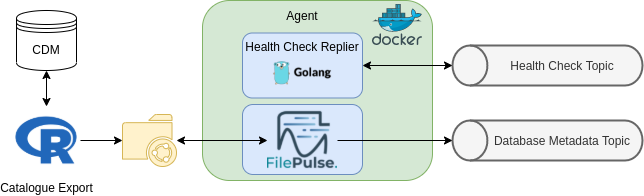
\includegraphics[width=\textwidth]{agent-architecture}
    \caption{agent arch}
    \label{fig:agent-architecture}
\end{figure}

\section{Publishing}

data is in kafka. what do we have to do to reach the applications

\begin{itemize}
    \item need to send custom data on a CUSTOM FORMAT to a custom REST endpoint
    \item Kafka Sink Connectors (The target REST API is not customizable, such as the data format ) - need for a sender application
    \item No known end on kafka topics/streams - require some management on top of kafka
\end{itemize}

\section{Network Manager}  % change name
\begin{itemize}
    \item centralized entity
    \item transforms the data to the required format
    \item sends to the specific application's endpoint
    \item 5 components
\end{itemize}

\subsection{Pipelines Workers}
\begin{itemize}
    \item select and filter the data comming from the databses
    \item only process data of a single database at a time. handling multiple is the same is hard to handle and hard to scale
    \item scalable: several pipeline worker applications
\end{itemize}

\subsection{Orchestrator}
\begin{itemize}
    \item To ensure multiple records of multiple databases are not processes at the same time, this component redirects the data from databases to the pipelines workers preventing the previous problem
\end{itemize}

\subsection{Sender}
\begin{itemize}
    \item sends/publishes the data resulting from the pipelines, to the application's endpoints
\end{itemize}

\subsection{Admin Dashboard}
\begin{itemize}
    \item manage the whole thing
    \item Allows to create new pipelines and add aplications
\end{itemize}

\subsection{Statistics Recorder}
\begin{itemize}
    \item Listens to the kafka topics that are used along the system and transforms into persistent data (sql)
\end{itemize}

\section{Network Data Flow}
\begin{itemize}
    \item Evaluation?
    \item step by step
    \item number of topics involved
\end{itemize}
